\documentclass[conference]{IEEEtran}

\usepackage[utf8]{inputenc}
\usepackage{graphicx}
\usepackage{array}
\usepackage{float}
\usepackage{booktabs}

\begin{document}

%-------------------------------------------------
% Title & Author
%-------------------------------------------------
\title{Informe de Laboratorio 1 \\
\large \textit{Aplicaciones electroindustriales}}


\author{
\IEEEauthorblockN{2\textsuperscript{nd} Mateo Lecuna }
\IEEEauthorblockA{\textit{Ingeniería en Mecatrónica} \\
\textit{Universidad Tecnológica (UTEC)}\\
Fray Bentos, Uruguay \\
mateo.lecuna@estudiantes.utec.edu.uy}
\and

\IEEEauthorblockN{1\textsuperscript{st} Hector Pereira}
\IEEEauthorblockA{\textit{Ingeniería en Mecatrónica} \\
\textit{Universidad Tecnológica (UTEC)}\\
Fray Bentos, Uruguay \\
hector.pereira@estudiantes.utec.edu.uy}
\and

\IEEEauthorblockN{2\textsuperscript{rd} Priscila Rossi}
\IEEEauthorblockA{\textit{Ingeniería en Mecatrónica} \\
\textit{Universidad Tecnológica (UTEC)}\\
Fray Bentos, Uruguay \\
priscila.rossi@estudiantes.utec.edu.uy}
}

\maketitle

%-------------------------------------------------
% Abstract
%-------------------------------------------------
\begin{abstract}
Inspección, completado, cableado, y operación de un motor trifásico de inducción con arranque estrella-triángulo.
\end{abstract}

%-------------------------------------------------
% Content (importing your sections)
%-------------------------------------------------
\section{Introducción}
En este laboratorio se trabajó con un sistema industrial sencillo compuesto por un motor trifásico de inducción de pequeña potencia y su tablero de comando y protección. 
El objetivo principal fue inspeccionar, completar el cableado y poner en funcionamiento la instalación, aplicando criterios de seguridad eléctrica y verificando el correcto desempeño del arranque estrella-triángulo.  

El trabajo incluyó la verificación del plano eléctrico (CadeSimu), la reconexión de los cables faltantes, la operación del circuito de comando y potencia, y la realización de mediciones de corriente y potencia.

<<<<<<< HEAD
\section{Marco teórico}
=======
\section{Marco Teórico}
\begin{itemize}
    \item \textbf{Motor de inducción trifásico}: convierte energía eléctrica en energía mecánica. Puede conectarse en estrella (380 V) o en triángulo (220 V).
    \item \textbf{Transformador trifásico}: adapta la tensión de red (400 V) a la tensión nominal del motor (230 V).
    \item \textbf{Arranque estrella-triángulo}: método que reduce la corriente de arranque y luego conmuta a triángulo para el régimen nominal.
    \item \textbf{Tablero de comando y protección (TCP)}: contiene interruptores, guardamotores, contactores y protección diferencial para maniobrar y proteger al motor.
    \item \textbf{Circuitos}: 
    \begin{itemize}
        \item Comando: señales de baja tensión (24 V CC).
        \item Potencia: alimentación del motor (230 V CA trifásica).
    \end{itemize}
    \item \textbf{Seguridad}: se trabajó inicialmente sin tensión, evitando contacto con niveles peligrosos.
\end{itemize}
>>>>>>> 35d0f89bce6080235d88bd3fc7ab7f6b081db0d8

\section{Metodología}
\subsection{Revisión de seguridad}

Antes de comenzar con cualquier actividad práctica se efectuó una verificación de las condiciones de seguridad, teniendo en cuenta que en este laboratorio se trabaja con tensiones eléctricas de diferentes niveles. Se identificó que el circuito de comando está alimentado por una fuente de 24 V en corriente continua, considerado como un nivel de tensión segura, ya que no representa riesgo de daño físico en caso de contacto accidental. En cambio, el circuito de potencia funciona con 230 V en corriente alterna trifásica, lo que constituye un nivel de tensión no seguro, capaz de provocar descargas y accidentes graves si se produjera un contacto directo.  

La principal medida de seguridad consistió en impedir cualquier contacto accidental con el circuito de potencia. Por esta razón, las primeras tareas de inspección y conexionado del tablero se realizaron con los equipos totalmente desconectados de la red trifásica. Sólo una vez que el docente autorizó, y luego de comprobarse que el cableado se encontraba en condiciones correctas, se procedió a energizar la instalación de forma controlada.  

También se revisó la presencia y el correcto funcionamiento de los dispositivos de protección integrados en el Tablero de Comando y Protección, como el interruptor automático, el guardamotor y el interruptor diferencial tetrapolar. Estos elementos resultan esenciales para garantizar la desconexión inmediata en situaciones de sobrecarga, cortocircuito o derivación a tierra, preservando así la seguridad de los estudiantes y la integridad de los equipos.

[Foto del circuito original]

\subsection{Inspección del cableado}

Con la instalación completamente desenergizada se procedió a realizar la inspección detallada del tablero de comando. El objetivo de esta etapa fue verificar el estado general del cableado, comprobar la correspondencia con el diagrama eléctrico suministrado y registrar la información necesaria para completar el plano de trabajo.  

Durante la revisión se prestó especial atención a la identificación de los conductores, la correcta fijación en bornes y regletas, y la continuidad de las conexiones en los circuitos de comando. Se constató además la presencia de las protecciones asociadas y se compararon los datos observados con la documentación proporcionada, lo que permitió reconocer qué partes del conexionado estaban faltantes, para luego proceder a volver a conectarlas.

[Foto del circuito armado]

\subsection{Energización y prueba operativa}

Una vez verificado el cableado y confirmada la correcta conexión de los conductores se procedió a energizar el tablero de manera controlada. La activación se realizó con la supervisión del docente, siguiendo una secuencia ordenada de habilitación de los interruptores principales y de protección, con el fin de evitar corrientes transitorias o maniobras indebidas.  

Al aplicarse la tensión trifásica de 230 V al Tablero de Comando y Protección, se encendieron los indicadores luminosos que confirmaron la disponibilidad del sistema para la puesta en marcha. A partir de este momento se efectuaron las primeras pruebas de operación del motor mediante las botoneras de arranque y parada, verificando que las órdenes de comando eran transmitidas correctamente y que no se presentaban fallos eléctricos en el proceso.  

Durante esta etapa se corroboró además el funcionamiento adecuado de los dispositivos de protección, asegurando que las condiciones de seguridad se mantuvieran en todo momento y que el motor respondiera de acuerdo a la secuencia prevista para su arranque y detención.

[Link al video del drive funcionando]

\subsection{Observación de la actuación}

Durante la operación del sistema se prestó especial atención a la secuencia de actuación de los elementos de mando y protección. Se observó el comportamiento de los contactores en el arranque y la conmutación prevista para el motor, así como la respuesta de las botoneras de encendido y apagado frente a cada orden de comando.  

El seguimiento de los indicadores luminosos permitió confirmar el estado de los distintos circuitos en tiempo real, verificando que las señales visuales coincidieran con la condición esperada del motor y del tablero. Esta observación fue fundamental para constatar que el esquema de arranque respondiera de acuerdo con el diseño, sin interrupciones ni fallos de sincronización.  

De esta manera, la supervisión directa de la actuación de los componentes no solo confirmó el correcto conexionado realizado en etapas anteriores, sino que también permitió adquirir una comprensión práctica sobre la lógica de control implementada en el sistema de arranque y protección del motor.

\subsection{Medición de corriente}

Con el motor en funcionamiento estable se procedió a la medición de las corrientes eléctricas en cada fase del circuito de potencia. Para esta tarea se utilizó una pinza amperimétrica, que permitió obtener valores instantáneos de corriente sin necesidad de interrumpir el circuito, y un analizador de energía del tipo Power Energy Logger, que complementó la información al registrar también la potencia eléctrica entregada al motor.  

[Valores medidos]

Las mediciones se realizaron en condiciones de régimen permanente, luego del arranque, para evitar que los picos transitorios propios de la puesta en marcha alteraran los resultados. Los valores obtenidos fueron registrados cuidadosamente en una planilla de trabajo en formato Excel, destinada a su posterior inclusión en el informe final.  

Estos registros permitieron evaluar el desempeño del motor bajo las condiciones de carga establecidas y verificar que los consumos eléctricos se mantuvieran dentro de los parámetros nominales indicados en la placa del equipo. Además, los datos recopilados servirán de base para la elaboración de conclusiones acerca de la eficiencia del sistema y del correcto dimensionamiento de los dispositivos de protección.

\section{Resultados}

En esta sección se presentan las evidencias obtenidas durante el desarrollo de la práctica, que permiten verificar el correcto funcionamiento del circuito de arranque del motor trifásico.

En primer lugar, se documentó el estado inicial del tablero mediante una fotografía del circuito original, donde se aprecian las conexiones relevadas y los componentes principales del sistema. Posteriormente, se registró en una segunda fotografía el tablero con el cableado completado y verificado, mostrando las modificaciones y correcciones realizadas por el equipo durante el laboratorio (Figura \ref{fig:circuito_completo}).

Para complementar la evidencia visual, se incluye un enlace a un video almacenado en Google Drive donde se observa la secuencia de arranque y detención del motor, junto con la actuación de los contactores y los indicadores luminosos del tablero. Este registro audiovisual constituye una prueba adicional del funcionamiento del sistema bajo condiciones reales de operación:

%\href{https://drive.google.com/tu-enlace}{\textbf{Ver video de funcionamiento}}

Finalmente, en la Tabla \ref{tab:mediciones} se presentan los valores medidos de corriente y potencia eléctrica del motor durante su funcionamiento en régimen permanente. Estos datos fueron obtenidos con pinza amperimétrica y con el instrumento Power Energy Logger, y constituyen la base para el análisis y las conclusiones posteriores.


\begin{figure}[H]
\centering
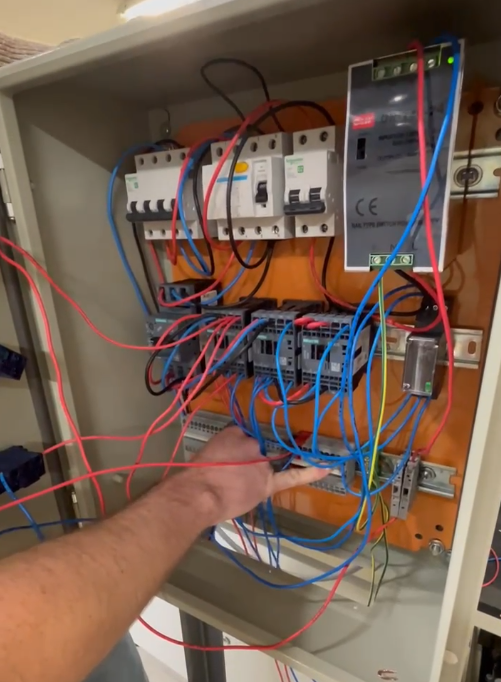
\includegraphics[width=0.4\textwidth]{anexos/circuitoCompleto.png}
\caption{Tablero con el cableado completado y verificado}
\label{fig:circuito_completo}
\end{figure}

\begin{table}[H]
    \centering
    \caption{Corriente medida según la configuración del motor.}

    \begin{tabular}{lc}
        \toprule
        \textbf{Configuración} & \textbf{Corriente (A)} \\
        \midrule
        Estrella (Y)  & 0.039 \\
        Triángulo ($\Delta$) & 0.098 \\
        \bottomrule
    \end{tabular}
\end{table}

%\begin{table}[H]
%\centering
%\caption{Valores de corriente y potencia medidos en el motor trifásico}
%\label{tab:mediciones}
%\begin{tabular}{|c|c|c|}
%\hline
%Fase & Corriente [A] & Potencia [W] \\
%\hline
%L1 & -- & -- \\
%L2 & -- & -- \\
%L3 & -- & -- \\
%\hline
%\end{tabular}
%\end{table}


\section{Conclusiones}
Comprobamos en banco que el tablero y el cableado responden a lo pedido: mando a 24~Vcc, potencia a 230~V trifásico (trafo 400/230~V) y secuencia de arranque estrella-triángulo con enclavamientos efectivos.

La puesta en marcha se realizó sin disparos ni golpes mecánicos; el temporizado elegido dio margen para que el motor tomara velocidad antes de conmutar.

El relevamiento y el ruteo final quedaron documentados en el diagrama ``conforme a obra'', lo que facilitó la verificación y el registro. Se identificaron con claridad los elementos de maniobra (K1, K2, K3 y el temporizador) y su correspondencia con el esquema.

En la práctica, el arranque en estrella redujo la exigencia eléctrica respecto del régimen en triángulo, en línea con la relación esperable $I_Y \approx I_\Delta/\sqrt{3}$. Las observaciones de potencia y factor de potencia fueron coherentes con la condición de prueba (sin carga o con carga ligera) y con el comportamiento típico de este método de arranque.

Como trabajo futuro, proponemos ajustar finamente $t_{Y\to\Delta}$ según la aplicación para suavizar aún más el transitorio, y registrar $I(t)$ durante el arranque para cuantificar el pico y comparar con el valor teórico. También conviene repetir las mediciones siempre sobre la misma fase en estrella y en triángulo para una comparación directa.


%-------------------------------------------------
% References
%-------------------------------------------------
\bibliographystyle{IEEEtran}
\nocite{*}
\bibliography{6_referencias.bib}

%-------------------------------------------------
% Appendix (optional)
%-------------------------------------------------

\section{Apendice}

\end{document}
